\chapter{INTRODUCTION}
\label{chapter:introduction}

\par
Software Testing is a broad field which is being already researched for more than 30 years and is applied by vast majority of software companies over the world. According to Pretschner et. al. Nowadays, half of overall development resources and time is spend for quality assurance which gives big motivation to optimize testing process and minimize time and cost of test design, development and execution so that quality of the product remains unharmed.

\par
Brainloop also is not an exception in this case. By giving the biggest concentration to security and quality of their products, they don't spare resources for testing. Including the Unit and Integration tests which are created by developers, nearly 50\% of the team resource is spend for testing. Brainloop is always open to the new approaches and trends for optimizing processes and wants to give a try to \acrlong{mbt} approach for one of its product: iOS application called Brainloop Secure Client.

\par
This chapter is divided into five sections. In section 1, we will describe implementation of Agile Scrum in Brainloop. We will discuss the current testing process in company, in section 2. In section 3 we will describe the motivation for this thesis which outlines the improvements which can be done in current testing process. Section 4, will introduce the requirements we need to fulfill by provided implementation for problems mentioned in section 3. In section 5, we will explain concept of \acrlong{mbt} and discuss different approach which can be applied during implementing it as well as shorcomings and adventages of each of them. The last chapter will explain the structure of the thesis.

\section{Agile Scrum in Brainloop}

\par
As a process for software development Brainloop has chosen agile Scrum. Small agile teams consist of product owner, developers, quality engineers and a scrum master. Product Owner is responsible for delivering well thought and fully described requirements in form of User Story. Developers are responsible for full implementation of the user story, including unit and integration tests. Quality Engineers are responsible for documenting test cases for verifying feature functionality and GUI correctness according to acceptance criteria of user story, editing any other previously documented test case which needs to be adjusted according to new user story, automating and executing manually documented test cases and also running exploratory tests against new feature. Scrum Master is responsible for solving any kind of impediments which team members might have during the development or testing, also optimizing the process within the team.

\par
Whole team together is obliged to deliver software increment in one sprint which in Brainloop is 2 weeks. During the sprint, couple of team meetings take place which are of vital importance for scrum process in Brainloop. These meetings are refinement, planning, retrospective and iteration review. During the refinement meeting, product owner introduces new user stories to the team, where team members discuss points around user story, raise questions regarding it and after raising points if the team is satisfied with the provided solutions and there are no impediments regarding this specific user story, it is refined and team accepts it. Next meeting is planning, where refined user stories get estimated and based on team capacity they are included into the next sprint. During retrospective team members are discussing what was beneficial and harmful during the sprint and providing this information to scrum master, who is responsible for resolving harmful issues. Iteration review takes place at the end of every sprint, where all teams shown their delivered increment to other teams and management.

\section{Current Testing Process in Brainloop}

\par
During the sprint quality engineers' work consists of couple of duties, which are documenting test cases, executing them manually and automating them as well. 
Documenting test cases includes in it analyzing the acceptance criteria of user stories included into the current sprint and documenting test cases thought by him or her into the issue tracker software. Along with this, quality engineer needs to keep track of previously documented test cases and alter those which are affected by the acceptance criteria of new user story.

\par
After documenting test cases, quality engineer needs to execute documented test cases against \acrlong{aut} in different environments, such as different operating systems, different devices, different server versions etc. Quality engineer needs to make sure as well that already implemented functionality of \acrlong{aut} remains stable and it is not broken by provided increment. For this he or she needs to execute Regression test plan which usually includes majority of the documented test cases for the whole functionality of the \acrlong{aut}. In case if quality engineer finds inconsistency between expected behaviour and actual behaviour of \acrlong{aut}, it needs to be documented in the issue tracker software as bug. Bug needs to have clear and explicit reproduction steps, needs to include log files from \acrlong{aut} and the information about environment where it got reproduced. After the bug is fixed by developers, tester's job also includes verifying that it is not reproducible any more.

\par
According to his or her capacity, quality engineer also needs to include test automation tasks into the sprint. In scope of this task, tester needs to automate test execution with predefined test execution software or framework, verify that automated test run is stable and does not provide false positive or true negative results.

\par
To illustrate description above, current testing process looks like figure below.

\begin{figure} [htbp!]
	\centering
					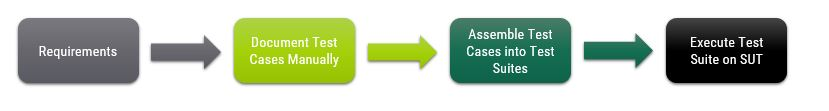
\includegraphics[width=1.1\textwidth]{figures/current_testing_process_flow.JPG}
					\caption{\label{Fig:current_testing_process_flow} Current Testing Process Flow}
\end{figure}

\section{Motivation}

\par
Even though testing process is quite fast, agile and is able to detect most of the bugs before the release, It can still be optimized by addressing the issues described below.

\par
Test cases are documented in static form, describing execution actions and expected results in plain English. They don't have any binding between each other, other than referencing, so similar kind of test cases involve lots of copying and pasting same text between each other, which brings up problem of their maintainability. When there is huge number of test cases which needs to be altered due to change in requirements, it takes significant time from testers' capacity to adjust these test cases to new requirements.

\par
Even if newest trends of test automation patterns, such as Keyword Driven Automation or Page Object Pattern are applied, tester still needs to create test modules for each test case separately, which needs to be adjusted to new requirements as well when it is required. Also, each of them need to have setup and teardown modules, ensuring the predefined starting and ending state of the test. This significantly increases execution time of each test and makes it less realistic compared to real customer use.

\par
In case of UI and Functional tests it is very difficult to talk with exact numbers in terms of coverage. When testers think of possible test cases for specific user story, they do their best to examine functionality from different perspectives, with different permission sets etc. At the end, generation of test cases are bound to the creativity of every quality engineer and does not make sure that all “Good” test cases (one which detects potential failure with good cost-effectiveness) are documented and executed.

\par
When there is a single unchanged regression test suite for \acrlong{aut}, which only gets incremented with test cases for new user stories, software gets resistant to this test suite and it stops finding new bugs, because all the bugs which it could have found are already fixed. This problem is known as Pesticide Paradox.

\par
For addressing above mentioned issues, \acrlong{mbt} comes into the picture with opportunity to automate not only the test execution but also the test design and generation process. Therefore, company is interested to see the results and improvements regarding quality, time and cost that can be achieved with this new approach.

\par
To sum up, Goal of this thesis is to give Brainloop information based on a research and case study, which will indicate how model-based testing will fit to the company’s agile environment, whether the change from existing testing process to model-based testing will improve the software quality and will be cost-effective.

\section{Requirements}

\par
The main requirement from Brainloop is that new approach should be usable by all quality engineers in the company. As testers are mostly involved in test design and execution process, they are not obliged to be proficient with any programming language or programming basics itself. So, to translate the requirement, the chosen approach and tool for implementing \acrlong{mbt} in Brainloop needs to be as much User Friendly as possible, preferably needs to have GUI for modelling and test generation as well, so that less training is needed for quality engineers to adopt \acrlong{mbt}.

\section{Model-Based Testing}


\par
description of MBT


\begin{figure} [htbp!]
	\centering
					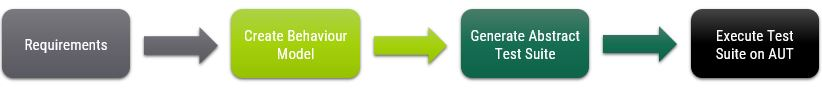
\includegraphics[width=1.1\textwidth]{figures/MBT_Flow.JPG}
					\caption{\label{Fig:MBT_Flow} Model-Based Testing Flow}
\end{figure}

\subsection{Off-line Model-Based Testing}
\subsubsection{Pros}
\subsubsection{Cons}
\subsection{On-line Model-Based Testing}
\subsubsection{Pros}
\subsubsection{Cons}

\section{Structure of the Thesis}
The thesis has been organized in a straightforward and effective manner to ease understanding. The flow of the thesis is described below:

\begin{enumerate}

\item \textit{Literature Review: }
Purpose of this chapter is to show investigations done for choosing the modeling approach and tool, which will fit most for the Brainloop Secure Client’s behaviour model. We review different modeling paradigms available for \acrlong{mbt} as well as the tools used by different researchers or companies to apply \acrlong{mbt} according to their needs. At the end of the chapter, justification will be provided regarding chosen paradigm and tool and how it fulfills our requirements and needs.

\item \textit{Modeling: } This chapter will provide information regarding our \acrlong{aut}, will describe the purpose of it's use and will give detailed information about modeling the behaviour of each part of the application.

\item \textit{Test Generation: } In this chapter, we will discuss different test generation criterions provided by our chosen tool, also you will find justification why it makes more sense to structure models in layers and also you will find definition of \acrshort{mrp} (\acrlong{mrp}) which was introduced in scope of this thesis.

\item \textit{Test Execution and Results: } This chapter provides information regarding execution effort of generated tests together with numbers of found issues during the test execution. Besides that, you will find comparison of results from current testing process to our results and explanation, why some issues were detected by former testing process and not by latter as well as explanation about opposite statement.

\item \textit{Conclusion:  }In this chapter, we will summarize effort and results of applying \acrlong{mbt} for Brainloop Secure Client. We will describe the vision about how \acrlong{mbt} can be integrated into the current Scrum process in Brainloop so that transition from current testing process to \acrlong{mbt} is smooth and we will describe the lessons learned during the thesis.

\item \textit{Limitations and future work: } In this chapter, we finish this study by addressing few limitations of our testing approach. We also discuss the enhancements and improvisations that can be fulfilled regarding application of \acrlong{mbt} in the future, which regrettably could not be addressed in this thesis.

\item \textit{Meta information: }In the further chapters, we have tabulated all the terminologies used throughout the report in more detail which may not be known to a layman and a few abbreviations that have been used.
    
\end{enumerate}
